\subsection{Kết quả tổng}
\label{sec:res-main}

\begin{table}[htbp]
\centering
\caption{Kết quả trên toàn bộ validation (\NVal{} câu; nguồn: \code{results/eval\_*\_validation.json})}
\label{tab:main}
\renewcommand{\arraystretch}{1.18}
\footnotesize
\setlength{\tabcolsep}{4pt}
\begin{tabularx}{\textwidth}{@{}L r r r r r r r@{}}
\toprule
& \multicolumn{2}{c}{\textbf{Toàn bộ}} & \multicolumn{2}{c}{\textbf{Có đáp án}} & \textbf{Không đáp án} & \textbf{Tỉ lệ} & \textbf{Độ trễ} \\
\cmidrule(lr){2-3}\cmidrule(lr){4-5}\cmidrule(lr){6-6}
\textbf{Hệ thống} & \textbf{EM} & \textbf{F1} & \textbf{EM} & \textbf{F1} & \textbf{EM} & \textbf{từ chối} & \textbf{ms/câu} \\
\midrule
\tabinput{generated/tab_main.tex}
\bottomrule
\end{tabularx}
\end{table}

\begin{figure}[htbp]
\centering
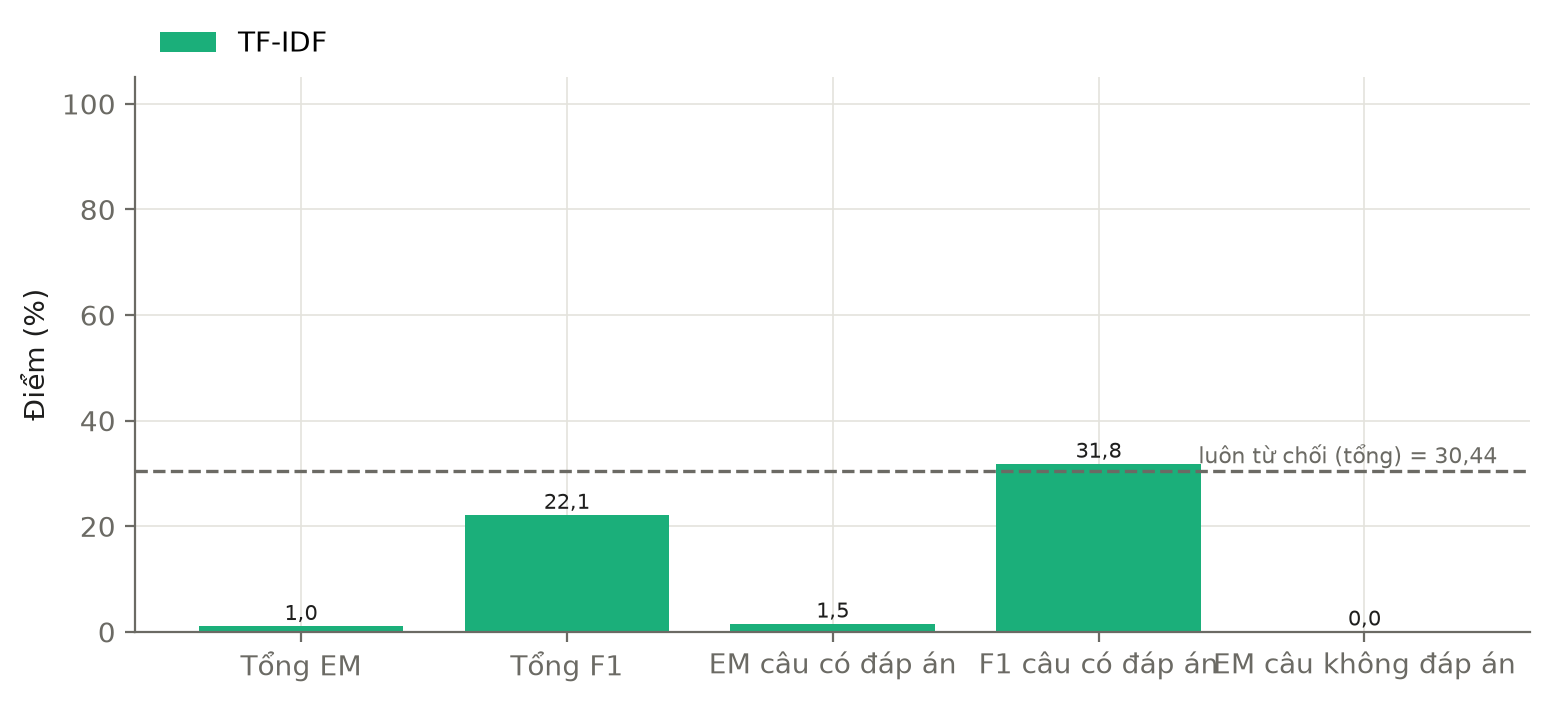
\includegraphics[width=\textwidth]{figures/main_results.png}
\caption{Kết quả chính. Đường đứt: điểm tổng của hệ thống luôn từ chối}
\label{fig:main}
\end{figure}

%RESULTS-MAIN-PROSE

\subsection{RQ1 --- Mô hình word-level có nhạy với ranh giới từ hơn?}
\label{sec:res-rq1}

\begin{table}[htbp]
\centering
\caption{EM/F1 theo tương thích biên từ của đáp án vàng (câu có đáp án)}
\label{tab:alignment}
\renewcommand{\arraystretch}{1.15}
\small
\begin{tabular}{@{}l r r r r@{}}
\toprule
& \multicolumn{2}{c}{\textbf{Khớp biên (\SegAligned{} câu)}} & \multicolumn{2}{c}{\textbf{Lệch biên (\SegMis{} câu)}} \\
\cmidrule(lr){2-3}\cmidrule(lr){4-5}
\textbf{Hệ thống} & \textbf{EM} & \textbf{F1} & \textbf{EM} & \textbf{F1} \\
\midrule
\tabinput{generated/tab_alignment.tex}
\bottomrule
\end{tabular}
\end{table}

\begin{table}[htbp]
\centering
\caption{Phân loại lỗi trên toàn bộ validation (số câu; định nghĩa ở Bảng~\ref{tab:taxonomy-def})}
\label{tab:taxonomy}
\renewcommand{\arraystretch}{1.15}
\footnotesize
\setlength{\tabcolsep}{4pt}
\begin{tabularx}{\textwidth}{@{}L r r r r r r r@{}}
\toprule
\textbf{Hệ thống} & \textbf{Tổng lỗi} & \textbf{Từ chối sai} & \textbf{Trả lời sai} & \textbf{Biên thừa} & \textbf{Biên thiếu} & \textbf{Biên lệch} & \textbf{Sai vị trí} \\
\midrule
\tabinput{generated/tab_taxonomy.tex}
\bottomrule
\end{tabularx}
\end{table}

\begin{figure}[htbp]
\centering
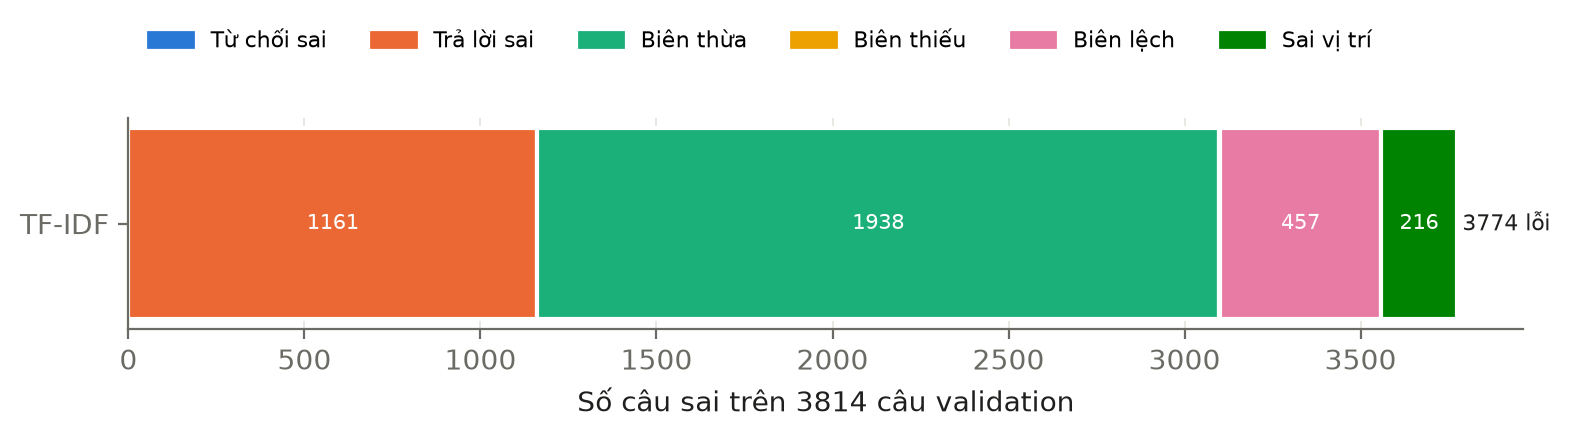
\includegraphics[width=\textwidth]{figures/error_taxonomy.png}
\caption{Cơ cấu lỗi của từng hệ thống}
\label{fig:taxonomy}
\end{figure}

\begin{table}[htbp]
\centering
\caption{So sánh cặp PhoBERT (A) và XLM-R (B) theo EM từng câu. Chênh lệch = EM(A) $-$ EM(B), điểm \%}
\label{tab:paired}
\renewcommand{\arraystretch}{1.15}
\footnotesize
\setlength{\tabcolsep}{4pt}
\begin{tabularx}{\textwidth}{@{}L r r r r r r l r@{}}
\toprule
\textbf{Nhóm câu} & $n$ & \textbf{Cả hai đúng} & \textbf{Chỉ A} & \textbf{Chỉ B} & \textbf{Cả hai sai} & \textbf{Chênh lệch} & \textbf{CI 95\%} & \textbf{$p$ McNemar} \\
\midrule
\tabinput{generated/tab_paired.tex}
\bottomrule
\end{tabularx}
\end{table}

%RESULTS-RQ1-PROSE

\subsection{RQ2 --- Độ dài ngữ cảnh và độ dài đáp án}
\label{sec:res-rq2}

\begin{table}[htbp]
\centering
\caption{EM / F1 theo độ dài đoạn văn (âm tiết). $^\dagger$: nhóm dưới 30 câu}
\label{tab:ctxlen}
\renewcommand{\arraystretch}{1.15}
\footnotesize
\begin{tabular}{@{}l r r r r r@{}}
\toprule
\textbf{Độ dài} & $n$ & \textbf{Luôn từ chối} & \textbf{TF-IDF} & \textbf{XLM-R} & \textbf{PhoBERT} \\
\midrule
\tabinput{generated/tab_context_length.tex}
\bottomrule
\end{tabular}
\end{table}

\begin{table}[htbp]
\centering
\caption{EM / F1 theo độ dài đáp án vàng (âm tiết; câu có đáp án)}
\label{tab:anslen}
\renewcommand{\arraystretch}{1.15}
\footnotesize
\begin{tabular}{@{}l r r r r@{}}
\toprule
\textbf{Hệ thống} & \textbf{1--2 (\NLenOne)} & \textbf{3--5 (\NLenThree)} & \textbf{6--10 (\NLenSix)} & \textbf{11+ (\NLenEleven)} \\
\midrule
\tabinput{generated/tab_answer_length.tex}
\bottomrule
\end{tabular}
\end{table}

\begin{figure}[htbp]
\centering
\begin{subfigure}{0.49\textwidth}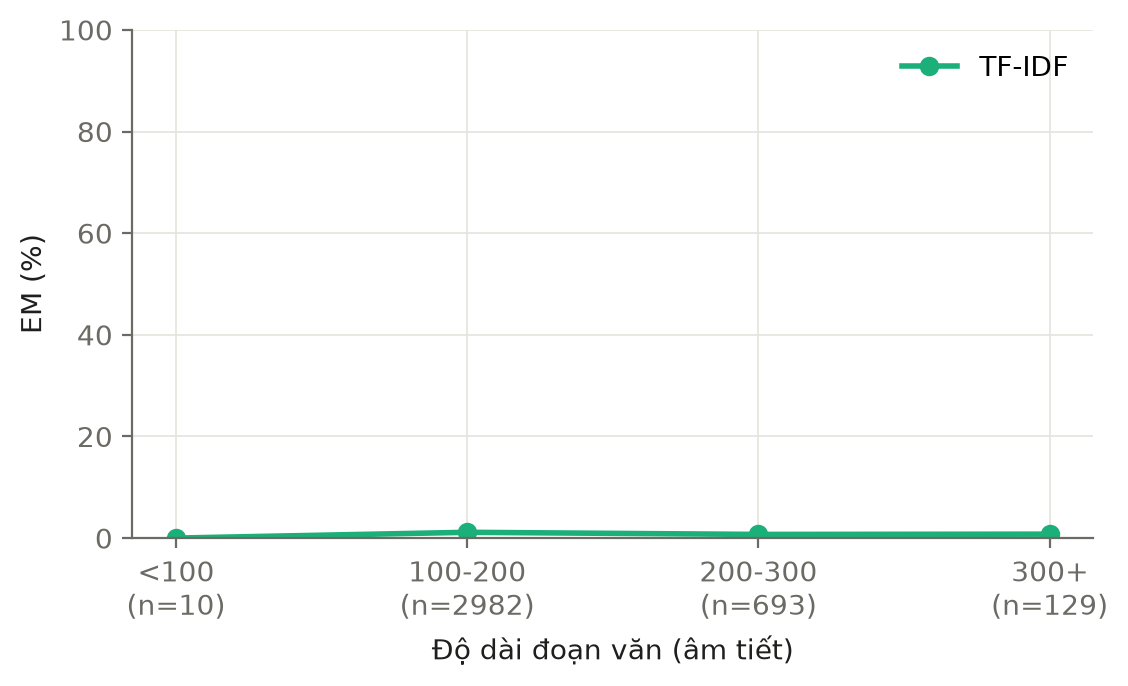
\includegraphics[width=\textwidth]{figures/by_context_length.png}\caption{Theo độ dài đoạn văn}\end{subfigure}
\hfill
\begin{subfigure}{0.49\textwidth}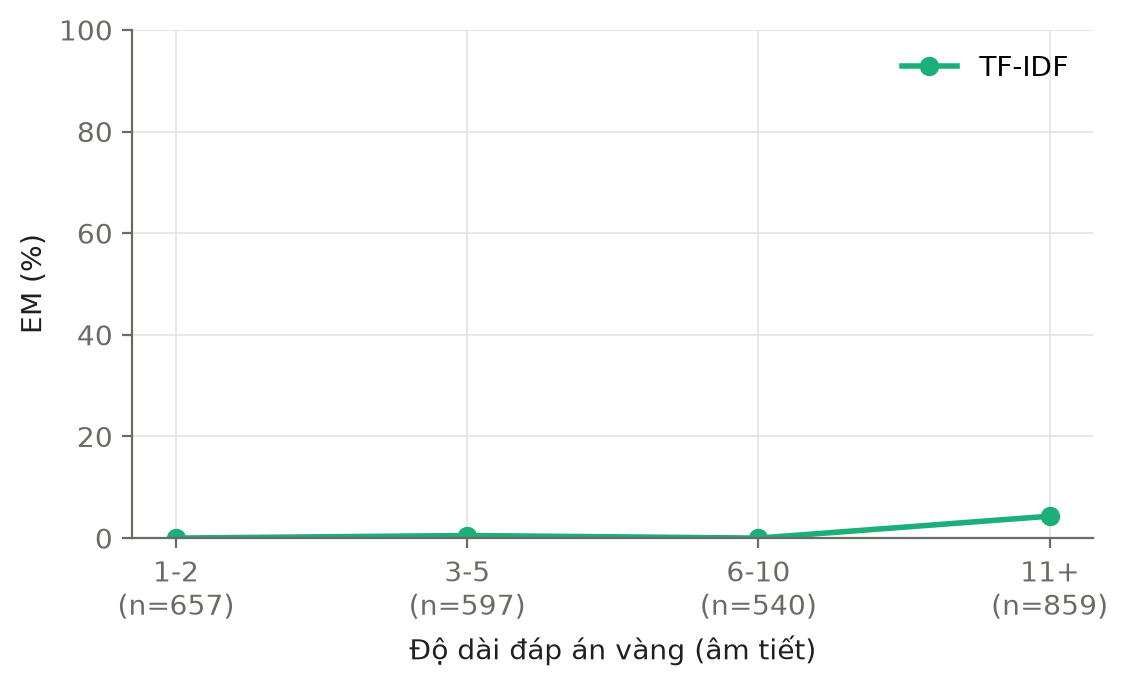
\includegraphics[width=\textwidth]{figures/by_answer_length.png}\caption{Theo độ dài đáp án}\end{subfigure}
\caption{EM theo độ dài}
\label{fig:lengths}
\end{figure}

%RESULTS-RQ2-PROSE

\subsection{RQ3 --- Nhận ra câu không có đáp án, hay thiên lệch về từ chối?}
\label{sec:res-rq3}

\begin{table}[htbp]
\centering
\caption{Hành vi từ chối như một bộ phân loại ``không có đáp án'' (validation)}
\label{tab:abstention}
\renewcommand{\arraystretch}{1.15}
\small
\begin{tabular}{@{}l r r r@{}}
\toprule
\textbf{Hệ thống} & \textbf{Tỉ lệ từ chối (\%)} & \textbf{Precision (\%)} & \textbf{Recall (\%)} \\
\midrule
Luôn từ chối & \AbstainAbsRate & \AbstainAbsPrec & \AbstainAbsRec \\
XLM-R-base & \XlmrAbsRate & \XlmrAbsPrec & \XlmrAbsRec \\
PhoBERT-base-v2 & \PhobertAbsRate & \PhobertAbsPrec & \PhobertAbsRec \\
\bottomrule
\end{tabular}
\par\vspace{2pt}{\footnotesize Tỉ lệ câu không có đáp án thật: \PctValImp\%.}
\end{table}

\begin{table}[htbp]
\centering
\caption{EM trên bộ stress-test theo nhóm: \emph{toàn bộ} / \emph{chỉ câu hợp lệ}. Chỉ để minh hoạ --- xem Mục~\ref{sec:audit}}
\label{tab:stress}
\renewcommand{\arraystretch}{1.15}
\footnotesize
\setlength{\tabcolsep}{4pt}
\begin{tabular}{@{}l r r r r r r@{}}
\toprule
\textbf{Hệ thống} & \textbf{E1} & \textbf{E2} & \textbf{E3} & \textbf{E4} & \textbf{E5} & \textbf{Tổng} \\
\midrule
\tabinput{generated/tab_stress.tex}
\bottomrule
\end{tabular}
\par\vspace{2pt}{\footnotesize Số câu hợp lệ mỗi nhóm: E1 \AuditEOneValid, E2 \AuditETwoValid, E3 \AuditEThreeValid, E4 \AuditEFourValid, E5 \AuditEFiveValid.}
\end{table}

%RESULTS-RQ3-PROSE

\subsection{RQ4 --- Transformer có vượt baseline ở mọi nhóm?}
\label{sec:res-rq4}

%RESULTS-RQ4-PROSE

\subsection{Phân tích định tính}
\label{sec:qualitative}

%RESULTS-QUAL-PROSE

\subsection{Quá trình huấn luyện và chi phí}
\label{sec:curves}

\begin{table}[htbp]
\centering
\caption{Đường cong huấn luyện. EM/F1 đo trên dev (500 câu ngẫu nhiên tách từ train). $\star$: epoch được chọn}
\label{tab:curves}
\renewcommand{\arraystretch}{1.15}
\small
\begin{tabular}{@{}l c r r r r@{}}
\toprule
\textbf{Mô hình} & \textbf{Epoch} & \textbf{Loss} & \textbf{EM dev} & \textbf{F1 dev} & \textbf{Phút} \\
\midrule
\tabinput{generated/tab_curves.tex}
\bottomrule
\end{tabular}
\end{table}

\begin{figure}[htbp]
\centering
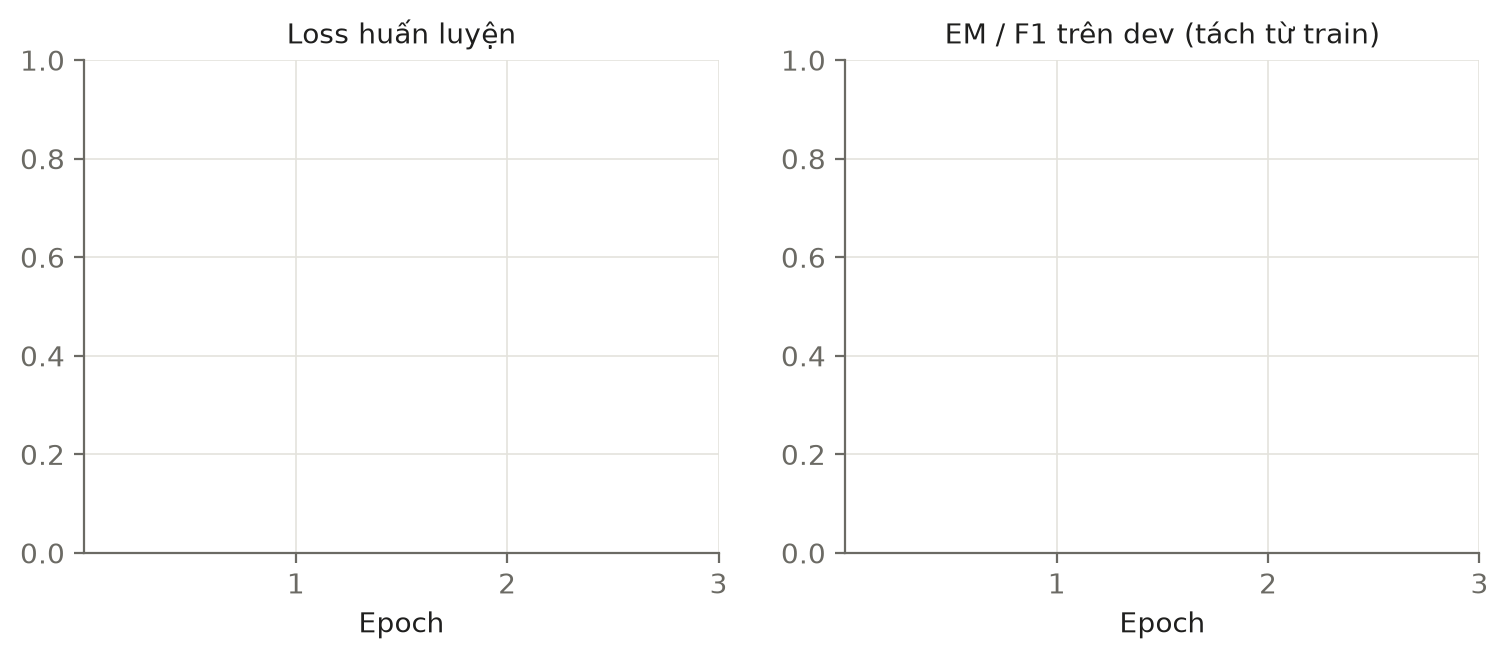
\includegraphics[width=\textwidth]{figures/training_curves.png}
\caption{Loss huấn luyện và EM/F1 trên dev theo epoch}
\label{fig:curves}
\end{figure}

%RESULTS-CURVES-PROSE
